\documentclass[11pt]{article}
%\renewcommand{\thesection}{\Roman{section}}  %zmiana section na rzymskie
\usepackage[utf8]{inputenc}
\usepackage[OT4]{polski}
\usepackage{tabularx}
\usepackage[margin=60pt]{geometry}
\usepackage{amsmath}
\usepackage{amsfonts}
\usepackage{listings} 
\usepackage[usenames,dvipsnames,table,xcdraw]{xcolor}
\usepackage{array}
\usepackage{sidecap} %do grafik
\usepackage{wrapfig} % j. w.
\usepackage{graphicx} %j.. w.
\usepackage{subfig} %j. w.
\usepackage{booktabs}
\usepackage{longtable}
\usepackage{hyperref}
\usepackage{nicefrac}
\usepackage{multirow}
\usepackage{siunitx}



\title{C.24 Model isinga ferromagnetyka}
\author{Paweł Rzońca}
\date{}
\begin{document}

\maketitle

\section*{Wstęp}

Dokładny opis projektu znajduje się na stronie \cite{strona}.

Dobrym roztóżnieniem pomiędzy różnymi magnetykami jest zachowanie się 
podatności magnetycznej $\chi$ wraz ze zmianą temperatury (\ref{pfa}). 
Dla ferromagnetyka 
w obszarze paramagnetycznym ($T \gg T_C$) spełnione jest prawo Curie-Weissa
\begin{equation}
\chi = \frac{C}{T-T_C},
\end{equation}
gdzie $T_C$ jest temperaturą Curie, a $C$ jest stałą.

\begin{figure}
\centering
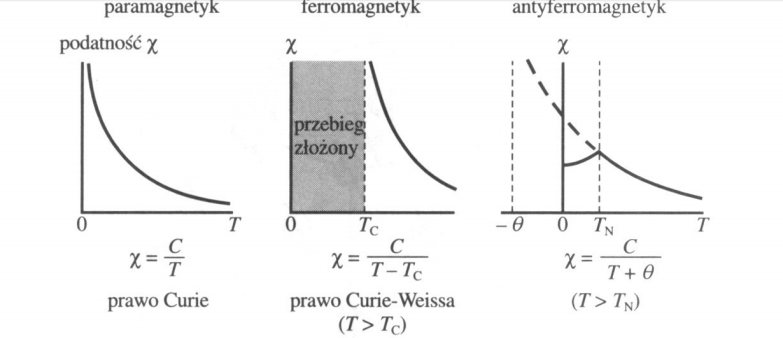
\includegraphics[width=0.6\textwidth]{pfa.png}
\caption{Podatność magnetyczna dla różych materiałów od temperatury materiału. 
Źródło \cite{Kittel}.}
{\label{pfa}}
\end{figure}


\section*{Metodyka}
W programie zaimplementowano algorytm podany w ćwiczeniu \cite{strona}.
Do przeglądania sieci wybrano metodę Monte Carlo. Za jeden krok MCS
(Monte Carlo Step) przyjęto sprawdzenie moliwości odwrócenia spinów w $N$ węzłach. 

We wstępnych fazach doświadczenia zbadano zachowanie układu 
w zależności od ilości kroków $N_{MC}$ Dla różnych wielkości 
siatki oraz różnych temperatur (wykresy \ref{MCvsLF} - \ref{MCvsTA}).

Widzimy iż układ osiąga porządany stan szybciej dla małych siatek. 
Oznacza to że z rozmiarem siatki musimy zwiększać ilość kroków 
co powoduje wydłużenie czasu obliczeń. Z tego względu zdecydowano się 
na siatkę o rozmiarze $32\times32$. Widzimy, iż układ ustala się 
we właściwej pozycji już po 150 MCSs. W doświadczeniach przyjęto 
siatkę o wielkości \textbf{32$\times$32} oraz \textbf{200 MCS}.
\begin{figure}
\centering
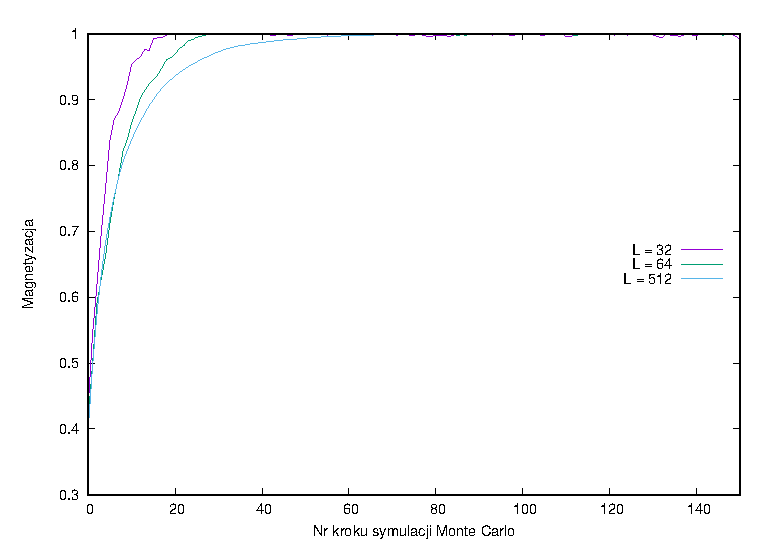
\includegraphics[width=0.6\textwidth]{MCvsLF.eps}
\caption{Porównanie szybkości stabilizacji układu dla różnych wielkości siatki
w przypadku ferromagnetyka $J=\SI{0.05}{\electronvolt}$ w temperaturze $kT=J$.}
{\label{MCvsLF}}
\end{figure}
\begin{figure}
\centering
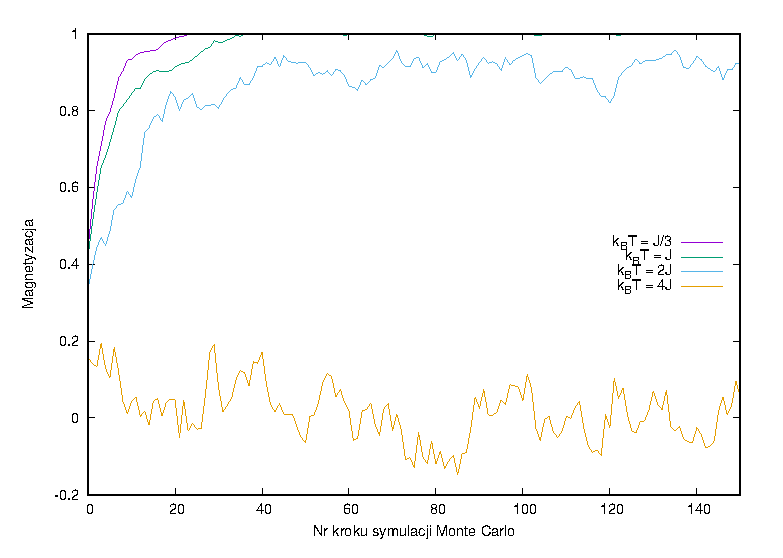
\includegraphics[width=0.6\textwidth]{MCvsTF.eps}
\caption{Porównanie szybkości stabilizacji układu dla różnych temperatur
w przypadku ferromagnetyka $J=\SI{0.05}{\electronvolt}$ przy siatce wielkości 
$32\times 32$.}
{\label{MCvsTF}}
\end{figure}
\begin{figure}
\centering
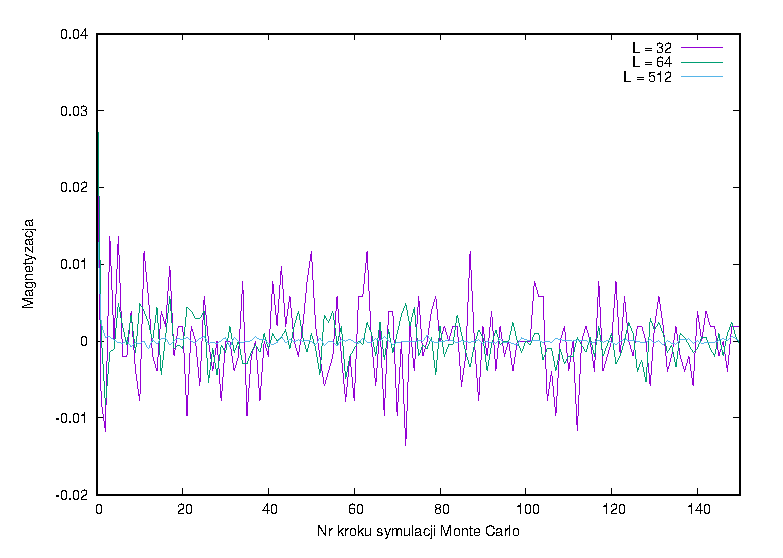
\includegraphics[width=0.6\textwidth]{MCvsLA.eps}
\caption{Porównanie szybkości stabilizacji układu dla różnych wielkości siatki
w przypadku antyferromagnetyka $J=\SI{-0.05}{\electronvolt}$ w temperaturze $kT=J$.}
{\label{MCvsLA}}
\end{figure}
\begin{figure}
\centering
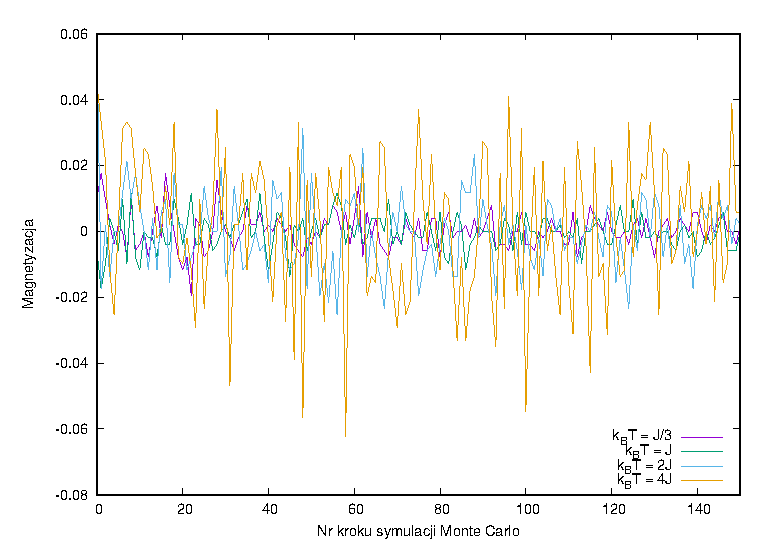
\includegraphics[width=0.6\textwidth]{MCvsTA.eps}
\caption{Porównanie szybkości stabilizacji układu dla różnych temperatur
w przypadku antyferromagnetyka $J=\SI{-0.05}{\electronvolt}$ przy siatce wielkości 
$32\times 32$.}
{\label{MCvsTA}}
\end{figure}
\section*{Wyniki}
\subsection*{Ferromagnetyk}
Sporządzono wykresy \ref{MvsTF} i \ref{MvsTF2} zależności magnetyzacji 
od temperatury dla ferromagnetykówo różnych całkach wymiany.
Widzimy, że skalując temperaturę czynnikiem $k/J$ otrzymujemy zawsze tę
samą temperaturę prejścia $T_C$ w okolicach $kT/J = 2-2,5$.
Oznacza to że temperatura Curie $T_C$ jest proporcjonalna do całki wymiany 
$J$.

Na wykresie \ref{MvsHF} widzimy zachowanie się modelu ferromagnetyka 
w polu zewnętrznym $H$ dla różnych temperatur. Dla niskich temperatur $T<T_C$
obserwujemy charakterystczną dla ferromagnetyka pętlę histerezy. Ze wzrostem 
temperatury pętla się zwęża.  Przy dostatecznie 
wysokiej temperaturze uporządkowanie znika i ferromagnetyk przechodzi w 
paramagnetyk (liniowa zależność od przyłożonego pola).

Następnie dla temperatur wyższych niż oszacowana $T_C = 2-2,5 J/k$ sporządzono 
wykres podatności magnetycznej od temperatury. Podatność magnetyczną 
wyznaczano ze wzoru $M (H) = \chi H$ w obszarze paramangetycznym 
gdzie zależność ta była liniowa. Do otrzymanych punktów dopasowano 
krzywą zgodną z prawem Curie-Weissa. Otrzymano w ten sposób wartość 
$T_C = 2,35 J/k$. Należy zaznaczyć iż wyznaczono niewiele punktów pomiarowych 
ze względu na długość obliczeń. 

\begin{figure}
\centering
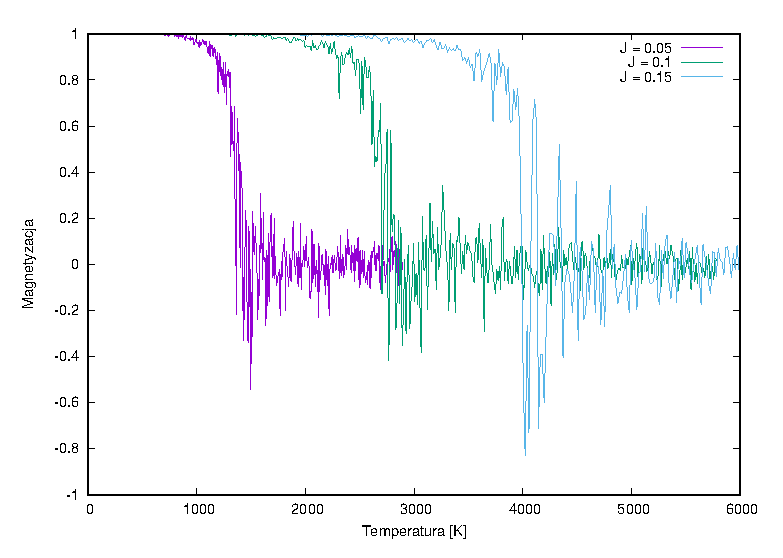
\includegraphics[width=0.6\textwidth]{MvsTF.eps}
\caption{Zależność magnetyzacji od temperatury dla ferromagnetyków.}{\label{MvsTF}}
\end{figure}
\begin{figure}
\centering
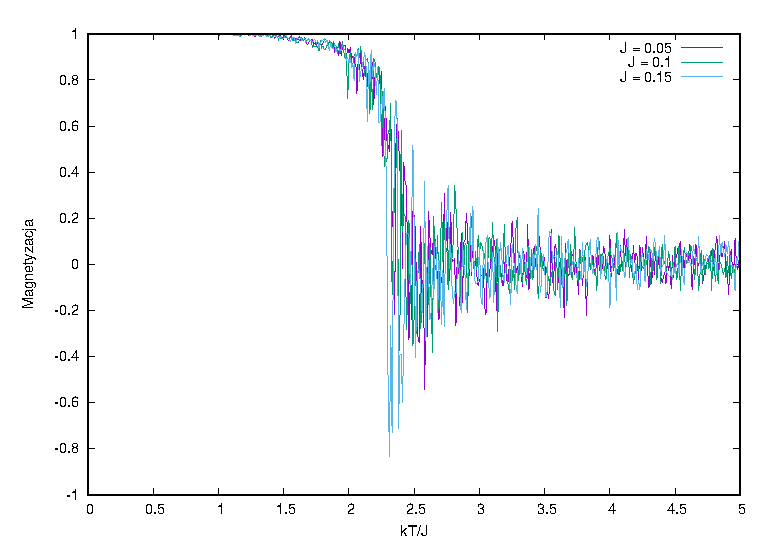
\includegraphics[width=0.6\textwidth]{MvsTF2.eps}
\caption{Zależność magnetyzacji od temperatury dla ferromagnetyków.}{\label{MvsTF2}}
\end{figure}
\begin{figure}
\centering
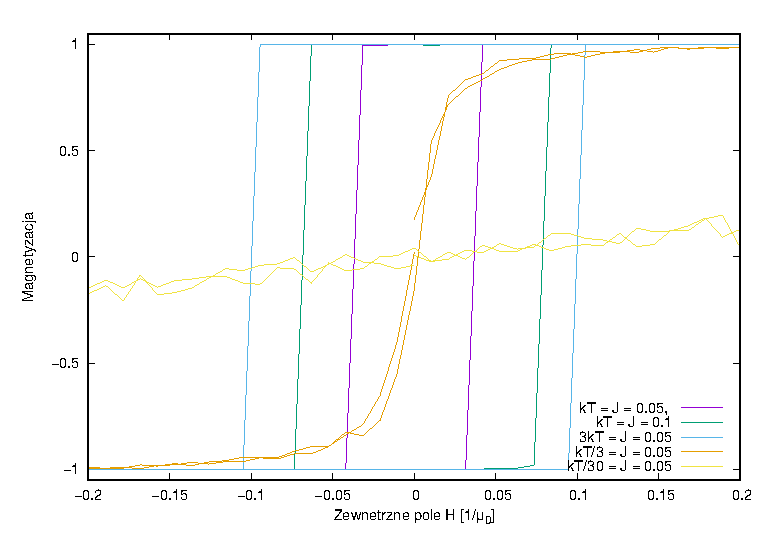
\includegraphics[width=0.6\textwidth]{MvsHF.eps}
\caption{Zależność magnetyzacji od pryłożonego pola 
$H$ dla ferromagnetyków.}{\label{MvsHF}}
\end{figure}
\begin{figure}
\centering
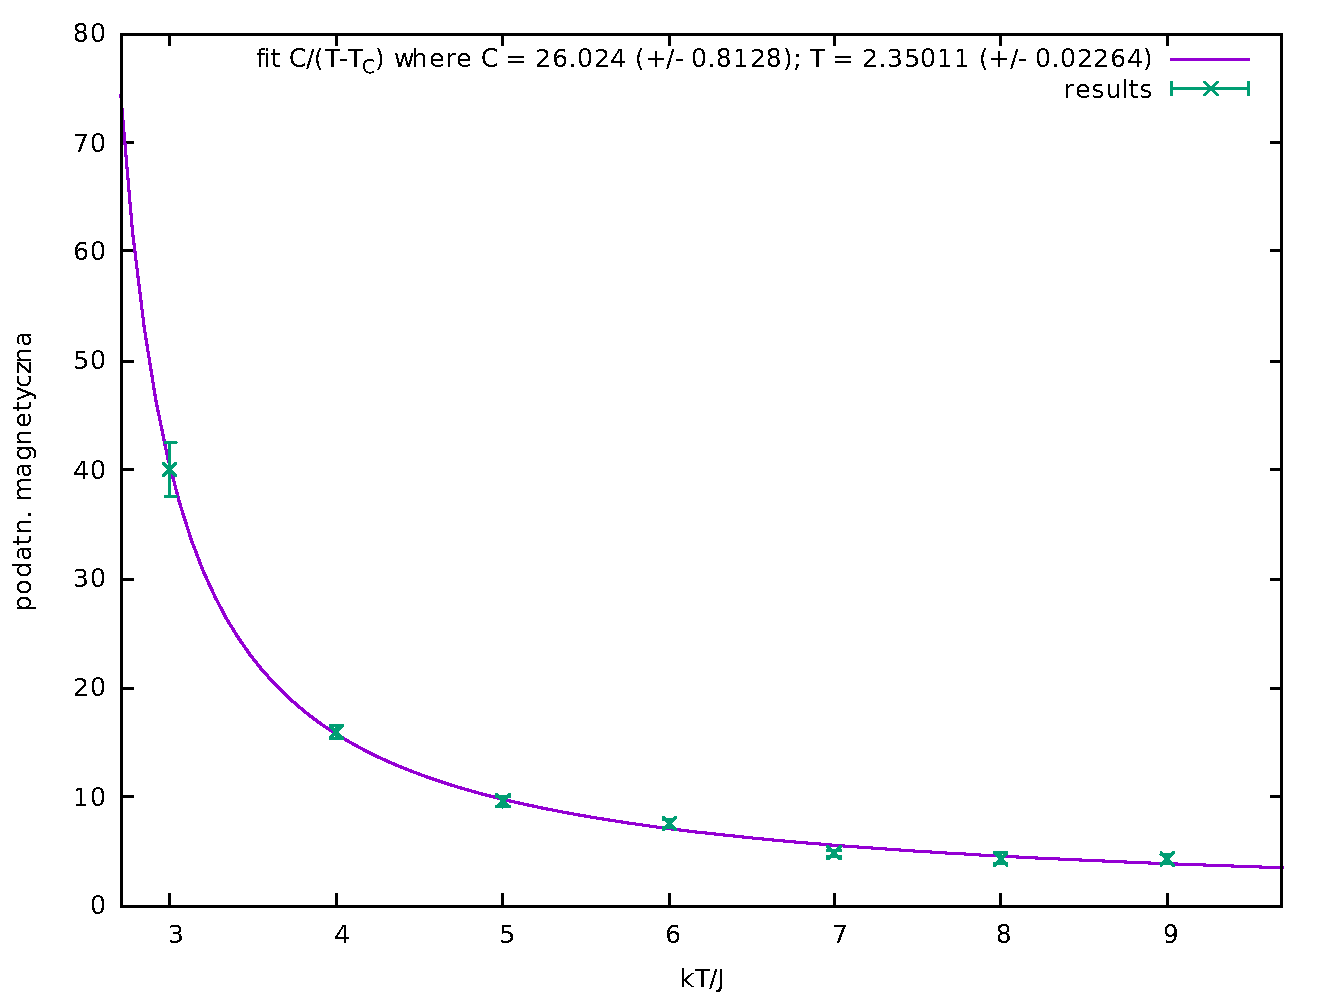
\includegraphics[width=0.6\textwidth]{CHIvsTF.pdf}
\caption{Zależność magnetyzacji od pryłożonego pola 
$H$ dla ferromagnetyków.}{\label{MvsHF}}
\end{figure}


\subsection*{Antyferromagnetyk}
Znalogicznie jak dla ferromagntyka wyznaczono zależność magnetyzacji od temperatury
(wykresy \ref{MvsTA} i \ref{MvsTA2}).
Analgicznie obserwujemy, że temperatura przejścia $T_N$ (Neela) jest proporcjonalna 
do całki wymiany $J$.

Wyznaczono również zależność magnetyzacji od przyłożonego pola (wykres \ref{MvsHA}).
Widzimy, że wraz z obniżaniem temperatury wykres robi się bardziej stromy. Tak jak poprzednio
przy dużych temperaturach przechodzi w paramagnetyka.

\begin{figure}
\centering
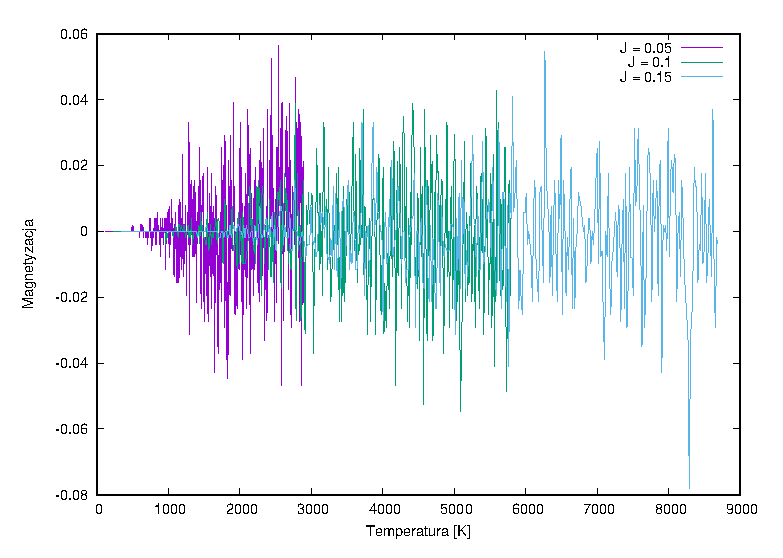
\includegraphics[width=0.6\textwidth]{MvsTA.eps}
\caption{Zależność magnetyzacji od temperatury dla ferromagnetyków.}{\label{MvsTA}}
\end{figure}
\begin{figure}
\centering
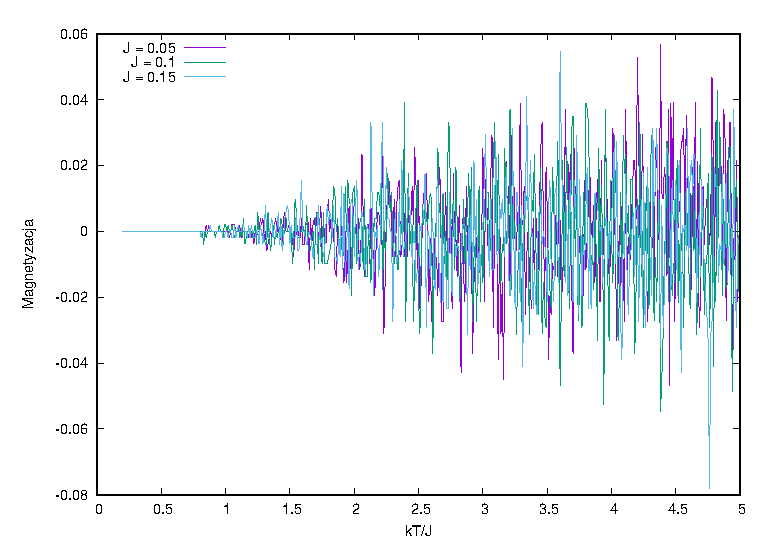
\includegraphics[width=0.6\textwidth]{MvsTA2.eps}
\caption{Zależność magnetyzacji od temperatury dla ferromagnetyków.}{\label{MvsTA2}}
\end{figure}
\begin{figure}
\centering
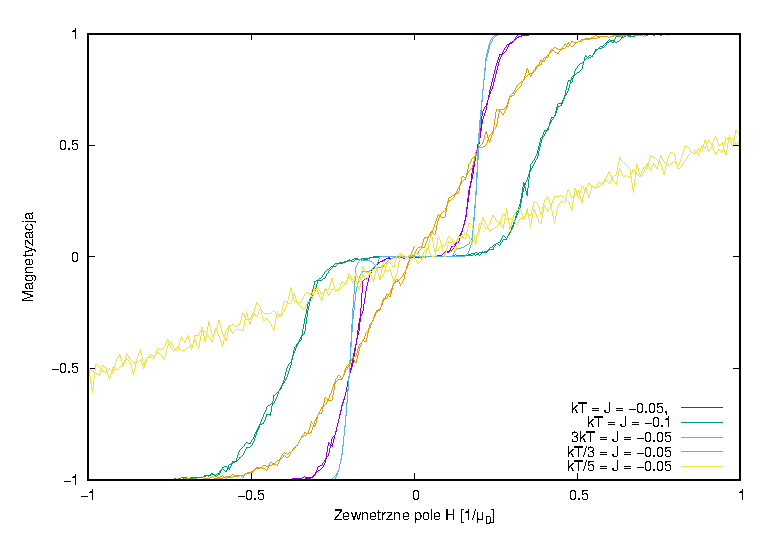
\includegraphics[width=0.6\textwidth]{MvsHA.eps}
\caption{Zależność magnetyzacji od pryłożonego pola 
$H$ dla antyferromagnetyków.}{\label{MvsHA}}
\end{figure}
%\begin{figure}
%\centering
%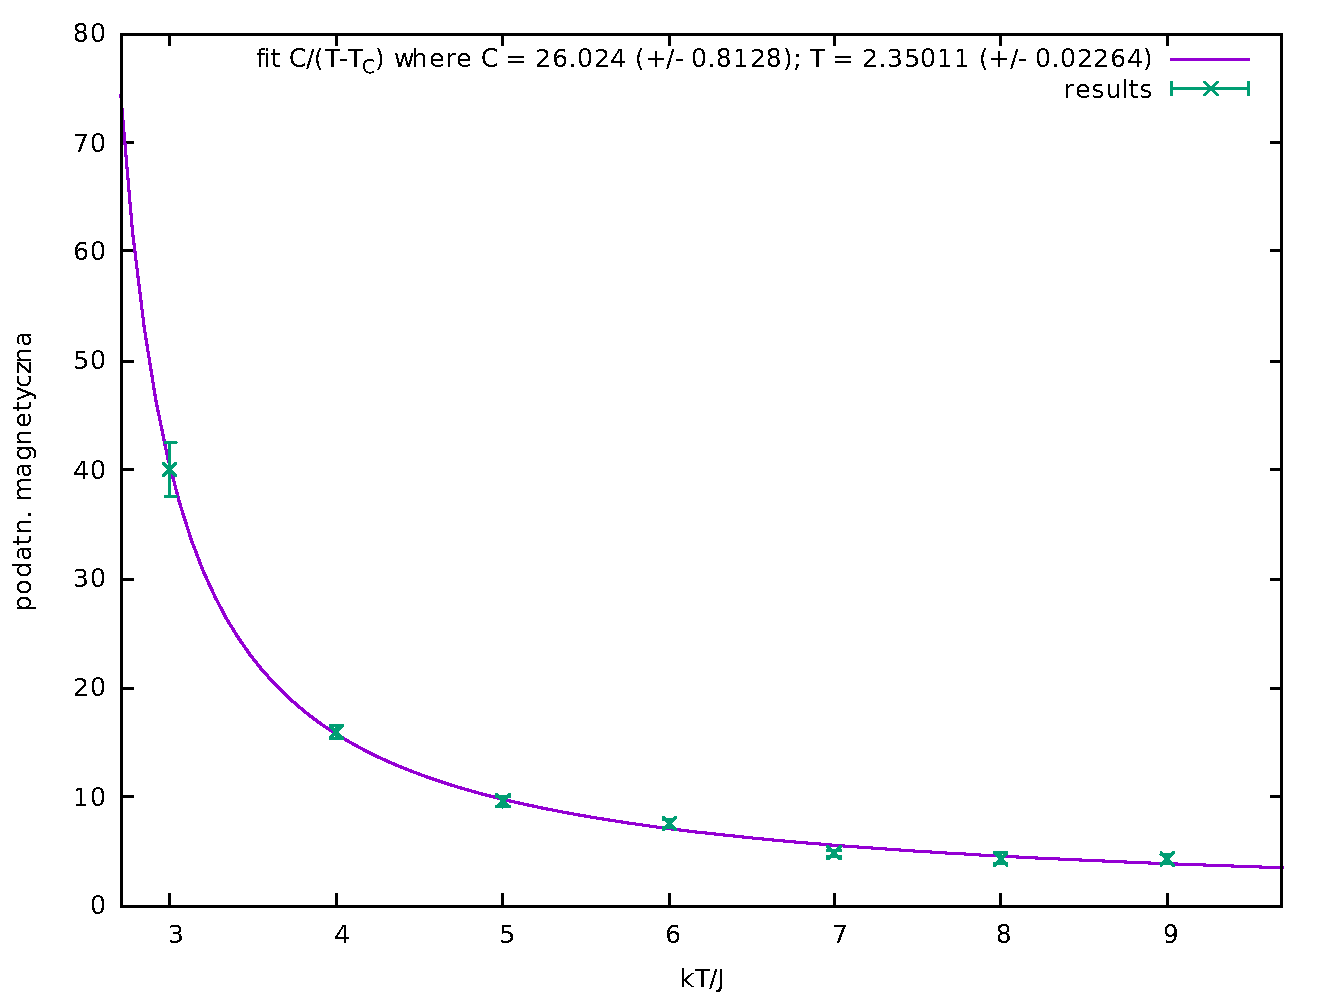
\includegraphics[width=0.6\textwidth]{CHIvsTF.pdf}
%\caption{Zależność magnetyzacji od pryłożonego pola 
%$H$ dla ferromagnetyków.}{\label{MvsHF}}
%\end{figure}

\section*{Podsumowanie}

W ćwiczeniu zaimplementowano model Isinga. Zbadano zależność magnetyzacji 
od temperatury oraz zewnętrznego pola zarówno w ferromagnetyku jak i antyferromagnetyku.
W niskich temperaturach momenty magnetyczne w ferromagnetyku ustawiają się równolegle, a
w ferromagnetyku antyrównolegle. Wykorzystując prawo Curie-Weissa wyznaczono temperaturę 
Curie ferroamgnetyka. 

\begin{thebibliography}{9}
\bibitem{strona}
    \url{http://newton.fis.agh.edu.pl/~wojcik/mof/mof1/Projekty_C.pdf}
\bibitem{Kittel}
    Charles Kittel, "Wstęp do fizyki ciała stałego", wydanie I, wyd. PWN, Warszawa 1999
\end{thebibliography}



\end{document}


